\documentclass[twocolumn,nofootinbib]{revtex4-1}
\usepackage{graphics}
\usepackage[caption=false]{subfig}
\usepackage{amsmath}
\usepackage{hyperref}
\usepackage{amssymb}
\usepackage{xcolor}
\usepackage{epsfig}
\usepackage{latexsym}
\usepackage{tensor}
\usepackage{float}
\usepackage{multirow}
\usepackage{xspace}
%\usepackage{wasysym}
\usepackage{comment}
\usepackage{acronym}
%\usepackage{graphicx}
%\usepackage{psfrag}

\graphicspath{{poster/figures/}}

%\newcommand{\gw}{gravitational wave }
%\newcommand{\gws}{gravitational waves }
\newcommand{\subgw}{_{\textrm{\scriptsize{GW}}}}
\newcommand{\ee}[1]{\ensuremath{\!\times\!10^{#1}}}
\newcommand{\prob}{{\rm Pr}}
\newcommand{\grbrate}{{{\mathcal R}_{\mathrm{grb}}}}
\newcommand{\cbcrate}{{{\mathcal R}}}
\newcommand{\diff}{{\mathrm d}}
\newcommand{\rhostar}{{\rho^*}}
\newcommand{\dhor}{\ensuremath{{\mathcal D}_{\mathrm{hor}}}}
\newcommand{\latin}[1]{\textit{#1}}
\newcommand{\mpc}{\mathrm{Mpc}}
\newcommand{\yr}{\mathrm{yr}}

\newacro{aLIGO}[aLIGO]{Advanced LIGO}
\newacro{GRB}[GRB]{gamma-ray burst}
\newacro{sGRB}[sGRB]{short gamma-ray burst}
\newacro{SGR}[SGR]{soft gamma-ray repeater}
\newacro{GW}[GW]{gravitational wave}
\newacro{NS}[NS]{neutron star}
\newacro{BH}[BH]{black hole}
\newacro{SNR}[SNR]{signal-to-noise ratio}
\newacro{MWEG}[MWEG]{Milky Way Equivalent Galaxy}
\newacro{KDE}[KDE]{kernel density estimation}
\newacro{MAP}[MAP]{Maximum \latin{a posteriori}}

\newcommand{\BNS}{\ac{NS}--\ac{NS}\xspace}
\newcommand{\NSBH}{\ac{NS}--\ac{BH}\xspace}
\newcommand{\JOINT}{\ac{GW}--\ac{sGRB}\xspace}

\def\imbh#1{intermediate mass black hole#1(IMBH#1)\gdef\imbh{IMBH}}
\def\smbh#1{supermassive black hole#1(SMBH#1)\gdef\smbh{SMBH}}
\def\bbh#1{binary black hole#1 (BBH#1)\gdef\bbh{BBH}}
\def\bh#1{black hole#1 (BH#1)\gdef\bh{BH}}
\def\sn#1{core-collapse supernova#1 (CCSN#1)\gdef\sn{CCSN}}
\def\pnw#1{post-Newtonian#1 (PN#1)\gdef\pnw{PN}}
\def\eos#1{equation of state#1 (EOS#1)\gdef\eos{EOS}}
\def\electro#1{electromagnetic#1 (EM#1)\gdef\electro{EM}}
\def\amr#1{adaptive mesh refinement#1 (AMR#1)\gdef\amr{AMR}}
\def\isco#1{innermost stable circular orbit#1 (ISCO#1)\gdef\isco{ISCO}}
\def\cwb#1{Coherent WaveBurst#1 (CWB#1)\gdef\cwb{CWB}}

\newcommand{\red}[1]{{\color{red}{#1}}}
\newcommand{\about}[1]{{\color{blue}{[THIS SECTION: #1]}}}
\newcommand{\add}[1]{{\color{magenta}{[TO INCLUDE: #1]}}}
\newcommand{\JC}[1]{{\color{magenta}{[[JC #1]]}}}
\definecolor{dwnote}{HTML}{E24A33}
\newcommand{\dwnote}[1]{{\color{dwnote}{[\textbf{DW}: #1]}}}
\newcommand{\placeholder}[2]{{\color{red}{[PLACEHOLDER](#1):}}{\color{red}{[}}#2{\color{red}{]}}}
\providecommand{\todo}[1]{{\color{red}$\blacksquare$~\textsf{[TODO: #1]}}}


\def\pasp{Publications of the Astronomical Society of the Pacific}
\def\mnras{Monthly Notices of the Royal Astronomical Society}
\def\aap{Astronomy and Astrophysics}


%%%%%% Useful for draft editing
\definecolor{dgreen}{rgb}{0.3, 0.73, 0.09}
\usepackage{soul} 
\usepackage{ulem} \normalem 
\newcommand{\ec}[1]{{\noindent\color{red}{\it [[#1]] }}}
\newcommand{\ish}[1]{{\color{blue}{#1}}}
\newcommand{\LC}[1]{{\color{red}{[[LC #1]]}}}
\newcommand{\AB}[1]{{\color{blue}{[[AB #1]]}}}
\newcommand{\highlight}[1]{\colorbox{yellow}{#1}}
\newcommand{\simgt}{\mbox{$^{>}_{\sim}$}}
\newcommand{\arw}[1]{{\color{dgreen}{#1}}}

\begin{document}

\title{Constraints On Short, Hard Gamma-Ray Burst Beaming Angles From
Gravitational Wave Observations}
\author{Daniel Williams, James Clark, Andrew Williamson, Ik Siong Heng, Martin Hendry}
\date{\today}

\begin{abstract}
\dots
\end{abstract}

\maketitle

\section{Introduction}
Gamma-ray bursts (GRBs)\acused{GRB} are extremely energetic
cosmological events observed at a rate of around one per day.  There
appear to be at least two separate populations of \acp{GRB}, divided
roughly according to their duration and spectral
hardness~\cite{Kouveliotou:1993yx}, although with significant overlap
obscuring any clear distinction between
populations~\cite{Zhang:2009uf,Bromberg:2012gp}.  Both types are
generally associated with systems which are also expected to be
\ac{GW} sources.  Those with long durations ($\gtrsim 2\,s$) and
softer spectra are associated with core collapse
supernovae~\cite{Galama:1998ea,MacFadyen:1998vz,Woosley:2006fn}, while
\acp{sGRB}, which exhibit on avergae harder spectra, are thought to be
related to compact binary coalescences involving at least one
\ac{NS}~\cite{Eichler:1989ve,Paczynski:1991aq,Narayan:1992iy,Lee:2007js}.

The detection of a \ac{GW} signal in coincidence with a \ac{GRB} would
provide tremendous insight in the astrophysics of these systems.  A
binary merger signal associated with an \ac{sGRB} would confirm the
compact binary merger nature of the engine and allow for measurements
of the binary component masses and spins, as well as constraints on
the beaming angles and the \ac{NS} equation of state.  Both \BNS and
\NSBH progenitors are possible, with the requirement that a post
merger torus of material accretes onto a compact central
object~\cite{Blandford:1977ds,Rosswog:2002rt,Giacomazzo:2012zt}.  A
population of \JOINT observations could allow us to measure the
fraction of \acp{sGRB} associated with each progenitor
type~\cite{Kreidberg:2012ud}.  A degeneracy between distance and
binary orbital inclination angle means that it will be difficult to
measure the \ac{sGRB} beaming angle based on a single observation.
However, with a population of binary merger sources, with and without
\ac{sGRB} counterparts, we can constrain the average opening
angle~\cite{Clark:2014jpa}.  A population of \JOINT observations with
associated redshifts will enable a relatively systematics-free
measurement of the Hubble parameter at low redshift, which would
provide constraints on cosmological
models~\cite{Schutz:1986gp,Chen:2012qh}.

In this work, we investigate what statements can \emph{currently} be
made on the beaming angle itself using the upper limits placed on
$\cbcrate$ from all-sky, all-time \ac{GW} searches and explore the
potential for direct inference of \ac{sGRB} beaming angles in the
advanced detector era.  We first discuss the relationship between
\acp{sGRB} and compact binary coalescences.  In particular, we will
focus on \BNS inspirals as the widely accepted progenitor for
\acp{sGRB}.  We then present our method for robustly inferring the jet
opening angles of \acp{sGRB}, using only \ac{GW} observations.  We
demonstrate our method assuming the nominal number of \ac{GW} signals
observed from \BNS inspirals expected for \ac{aLIGO} and Advanced
Virgo in planned \arw{`2017--2018' and `2022+'?} observing scenarios,
as defined in~\cite{Aasi:2013wya}.  We also show that our approach can
be used to place restrictions on the \ac{sGRB} jet opening angle if
there are no detections, and demonstrate this using results of the
recent first observing run of \ac{aLIGO}, during which no \BNS or
\NSBH signals were observed~\cite{Abbott:2016ymx}.  Finally, we
conclude with a discussion on the implications of our work as well as
possible avenues for further extension of the work presented here.


\section{Short gamma-ray bursts and compact binary coalescences}
\label{sec:sgrbs}
The compact binary coalescence hypothesis for \acp{sGRB} is supported
by a number of observations, notably: the large average separation of
\acp{sGRB} from their candidate host galaxies~\cite{Church:2011gk},
and the lower average star formation rate of these
hosts~\cite{Fong:2013eqa} --- suggesting old progenitor systems; their
short durations and rapid variability~\cite{Rees:1994nw} ---
suggesting very compact sources; and the observation of a kilonova
associated with GRB~130603B~\cite{Berger:2013wna,Tanvir:2013pia}.

At their design sensitivities, the current generation of advanced
\ac{GW} detectors could observe these mergers out to distances of
$\sim 400\,\mpc$ for \BNS or $\sim 1\,$Gpc for \NSBH, each at a rate of
$\sim 1\,$yr$^{-1}$~\cite{Aasi:2013wya}.  It is worth noting that at
galactic or near-galactic distances, \ac{SGR} hyperflares can resemble
\acp{sGRB}.  These \ac{SGR} hyperflares are the likely explanations
for GRB~070201 and GRB~051103, since compact binary coalescences at
the distance of their probable host galaxies were excluded with
greater than $90\%$ confidence \cite{Abbott:2007rh,Abadie:2012bz}.

Given the possible link between \acp{sGRB} and compact binary
coalescences, it is interesting to ask whether the \ac{sGRB} beaming
angle can be inferred from \ac{GW} observations.  For example, a
\JOINT observation could, in principle, constrain the beaming angle by
directly measuring the orbital inclination of the system.  As
discussed in~\cite{Clark:2014jpa}, however, the likely low \ac{SNR} of
such an observation coupled with the degeneracy between orbital
inclination and distance suggest that a comparison of the populations
of observed \acp{sGRB} and \BNS mergers may be more promising.
Motivated by the study in~\cite{2013PhRvL.111r1101C}, we note that if
the \ac{sGRB} population posseses a distribution of beaming angles
then the \emph{observed} rate of \acp{sGRB} is related to the rate of
\BNS coalescences $\cbcrate$ via,
%
\begin{equation}\label{eq:rate2angle}
    \grbrate = \epsilon\cbcrate \left \langle 1-\cos \theta \right \rangle,
\end{equation}
%
where angled brackets $\langle \rangle$ indicate the population mean
and $\epsilon$ is the probability that a binary coalescence results in
an observed \ac{sGRB}.  In this work, we assume
$\grbrate=10$\,Gpc$^{-3}$\,yr$^{-1}$~\cite{Nakar:2007yr,Dietz:2010eh}
and we shall refer to $\epsilon$ as the \ac{sGRB} \emph{efficiency}.
Generally, the efficiency with which \BNS mergers produce \acp{sGRB}
is unknown but will depend on a variety of progenitor physics.  In
particular, a significant fraction of \NSBH systems may be incapable
of powering an \ac{sGRB}~\cite{Pannarale:2014rea}.  Combining this
knowledge with measurements of the binary parameters of of a
population of\JOINT observations could be used to constrain
$\epsilon$.  In this work, we will make no attempt to characterize
$\epsilon$ and we simply aim to provide a framework which allows one
to incorporate various levels of assumptions (or ignorance) regarding
its value.

If the \ac{sGRB} population has a distribution of beaming angles, as
would seem likely from \electro{} observations, characterizing the
relative rates of \ac{sGRB} and \BNS coalescence will inform us as to
the mean of that population, $\langle \theta \rangle$.  To explore
this point further we construct a simple Monte Carlo simulation to
study the effect on the relative rates of \acp{sGRB} and \BNS mergers.
We arrange the following toy problem:
%
\begin{enumerate}
    \item Set the number of `observed \acp{sGRB} to zero: $N_{\mathrm{GRB}}=0$.
    \item Draw $N_{\mathrm{BNS}}$ values of orbital inclination $\iota$ from a distribution which is uniform in $\cos \iota$ in the range $[0,1]$.
    \item For each value of $\iota$, draw a value for the beaming angle $\theta$, from some distribution with finite width and limited to the range $(0,90]^{\circ}$.
    \item If $\iota<\theta$ then this combination of orbital inclination and beaming angle would result in an observable \ac{sGRB}, so increment $N_{\mathrm{GRB}}$.
\end{enumerate}
%
Such a simulation allows us to study the ratio of the number of
observed \ac{sGRB} to the total number of \BNS mergers
$N_{\mathrm{GRB}}/N_{\mathrm{BNS}}$.  Since it is the comparison of
the rates of these events that informs our inference on $\theta$,
studying the ratio $N_{\mathrm{GRB}}/N_{\mathrm{BNS}}$ provides some
intuition as to the effect and features of various $\theta$
distributions.  Figure~\ref{fig:thetapop} plots this ratio as a
function of various truncated normal distributions to demonstrate the
effect of shifting the mean and scaling the width of the distribution.
Points along the $x$-axis correspond to different choices of the
distribution width $\sigma_{\theta}$, and the separate curves
correspond to different choices of the distribution mean
$\langle \theta \rangle$.  Let us denote this truncated normal
distribution ${\mathcal N}(\langle \theta \rangle, \sigma_{\theta})$.
We stress here that such $\theta$ distributions are \emph{not}
intended to represent the true distribution; they are merely intended
to easily demonstrate the qualitative effects of different $\theta$
distributions on the ratio $N_{\mathrm{GRB}}/N_{\mathrm{BNS}}$.

\begin{figure}
\centering
%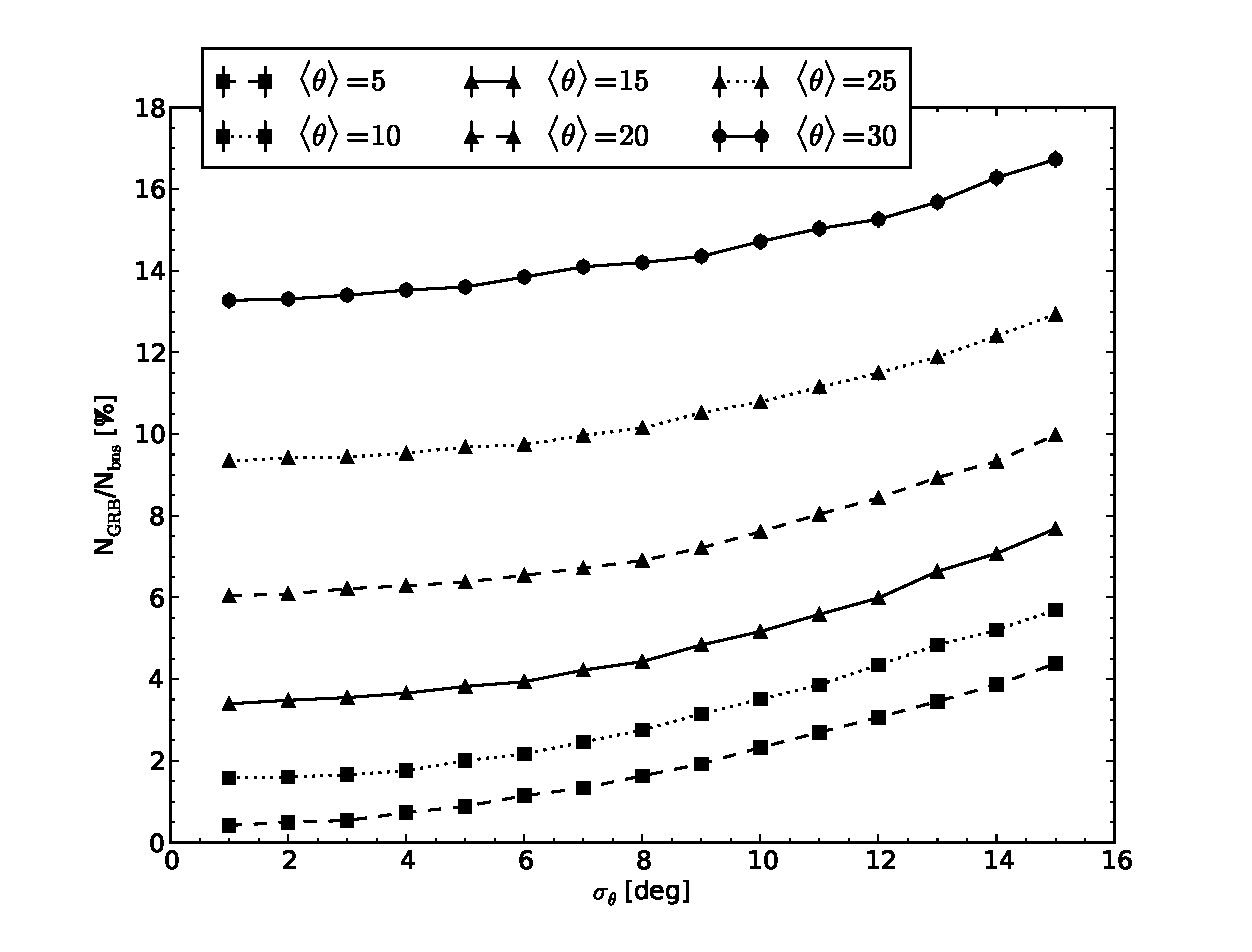
\includegraphics[width=\linewidth]{theta_dist_grbfrac.eps}
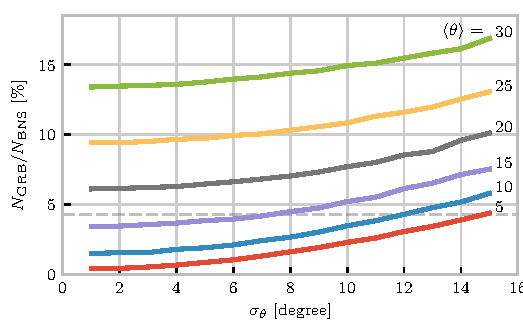
\includegraphics[width=\linewidth]{color_relativenumber.pdf}
\caption{\label{fig:thetapopulation} Expected relative
numbers of observed GRBs and binary coalescences for different distributions
on the GRB beaming angle.  Lines in the figure correspond to jet angle
population means, while the $x$-axis shows the width of the distribution.  All 
distributions are Gaussian, truncated at $(0, 90]$ degrees.\label{fig:thetapop}}
    % \centering
    % 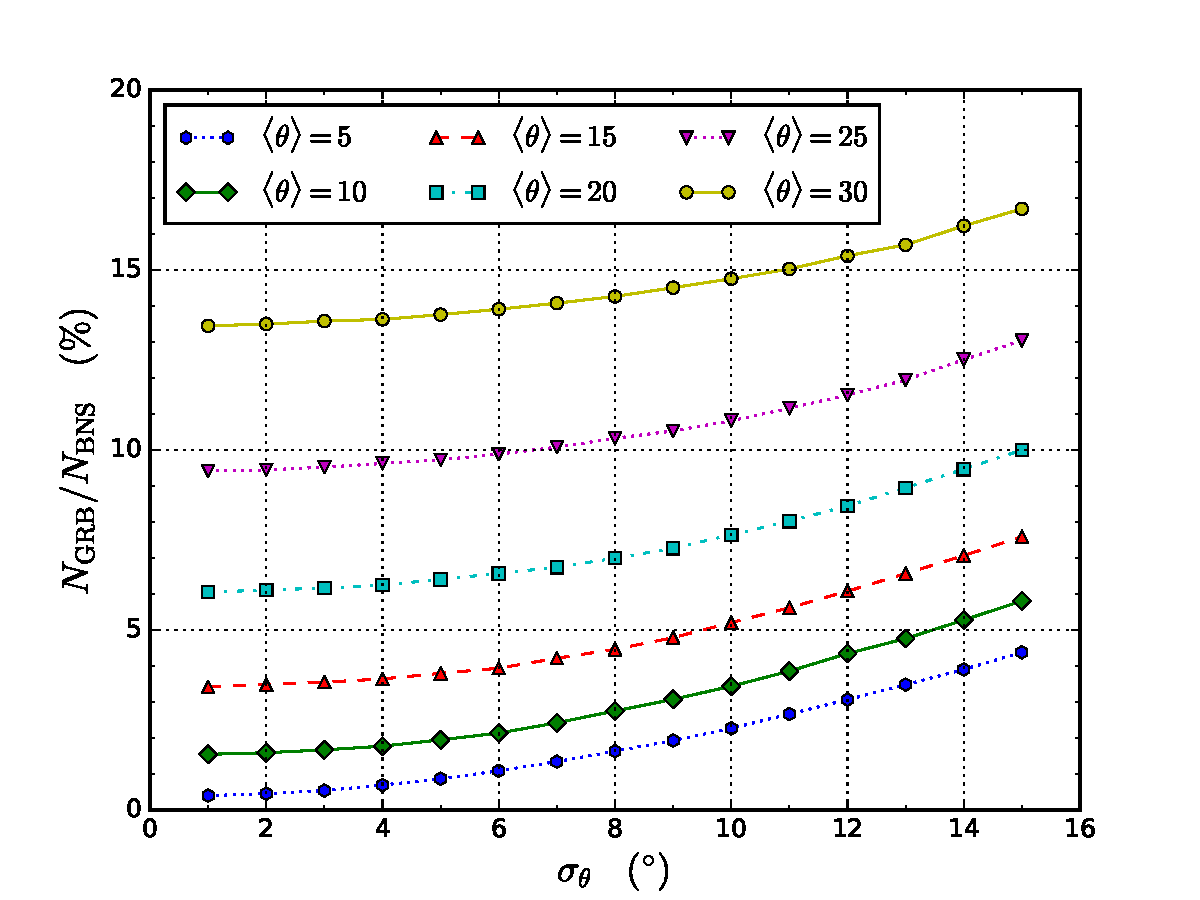
\includegraphics[width=\linewidth]{figure1.pdf}
    % \caption{Expected ratio of observed SGRBs and binary coalescences for different distributions on the SGRB beaming angle.
    %     For a series of jet angle population means, $\langle \theta \rangle$, we plot this ratio as a function of the distribution width, $\sigma_{\theta}$.
    %     All jet angle distributions are normal, truncated at $(0, 90]$ degrees.
    %     \label{fig:thetapop}}
\end{figure}




Figure~\ref{fig:thetapop} reveals that a population of \ac{sGRB} beaming angles with a large mean but narrow width is, on the basis of rate measurements, indidstinguishable from a population of \ac{sGRB} beaming angles with a small mean and large width.
For example, for the ${\mathcal N}(15,9)$ and ${\mathcal N}(10,13)$ beaming angle populations, the ratios of $N_{\mathrm{GRB}}/N_{\mathrm{BNS}}$ are almost equal ($\sim 4.8\%$).
Thus, a sufficiently wide spread of \ac{sGRB} beaming angles will yield relatively high rates for \BNS and \acp{sGRB} that could lead to an overestimate of the mean beaming angle.
The population-based constraints on $\theta$ must, therefore, be regarded as upper bounds on the mean of a distribution of beaming angles.
Having said this, for a given mean value $\langle \theta \rangle$, the ratio is rather insensitive to the width.


\section{From Rates To Beaming Angles}

In this section, we discuss our approach to estimating the \ac{sGRB} beaming angle based on the binary neutron star inspiral rate, estimated through a number of \ac{GW} observations of \BNS coalescence.
We demonstrate the approach by considering plausible detection scenarios for \ac{aLIGO}~\cite{Aasi:2013wya}.
Our ultimate goal is to develop a generic approach that folds in uncertainties in the \BNS merger rate and our ignorance about the probability with which such mergers actually result in \acp{sGRB}.
%
An overview of the general method is as follows:

\begin{enumerate}
    \item Estimate the posterior probability distribution on the \BNS merger rate
    in the local Universe from a number of observed gravitational wave signals
    and our knowledge of the sensitivity of the detectors.  We construct a joint
    posterior distribution on the \BNS rate and the (unknown) probability
    $\epsilon$ that a given merger results in a \ac{sGRB}.
\item Use equation~\ref{eq:rate2angle}, which relates the \BNS merger and
    \ac{sGRB} rates via the geometry of the beaming angle, to transform the rate
    posterior probability to a posterior probability on the mean \ac{sGRB}
    beaming angle.
\item Marginalize over $\epsilon$. We choose to consider $\epsilon$ a nuisance
    parameter because, to date, there is no accurate estimate of this parameter
    and it is not the main focus of our analysis. 
\end{enumerate}


\subsection{Constructing The Rate Posterior}
\label{sec:rate_posterior}
%   Gregory's book, `Logical Data Analysis For The Physical Sciences' has an entire
%   chapter (\S 14) devoted to `Bayesian Inference With Poisson Sampling'.  This
%   seems to match our problem rather well.  In particular, he derives expressions
%   for a Poisson rate posterior in \S 14.3, `Signal + known background' and \S
%   14.4, `Analysis of ON/OFF measurements' (``we want to infer the source rate, s,
%   when the background rate, b, is imprecisely measured'').
%
%It's tempting to jump straight into the On/off measurement stuff in \S~14.4 of
%Gregory, where the construction of the rate posterior includes the raw
%measurements of background rate.  I actually think this over-complicates things;
%if we wanted to do follow that procedure, we have to figure out the expected FAR
%for a given size of template bank etc.  There's a pretty well-established
%procedure for measuring this number: time-slides.  In fact, we don't even have
%to do any analysis.  Figure 3 (left panel) from the observing scenarios paper
%tells us everything we need to know.  Specifically, the following sentance has
%the information we need:

Our goal is to infer the posterior probability distribution for the mean
\ac{sGRB} beaming angle $\theta$ from \ac{GW} constraints on the rate of \BNS
coalescence $\cbcrate$.  The core ingredient to the analysis is the posterior
probability distribution on the coalescence rate $p(\cbcrate|D,I)$, where $D$
represents some \ac{GW} observation and $I$ denotes other unenumerated prior
information.  We will first demonstrate how $p(\cbcrate|D,I)$ may be constructed
for a few projected observing scenarios from~\cite{Aasi:2013wya}.  Later, in
section~\ref{sec:beaming_limits}, we will extend the analysis to place upper
limits on $\theta$ \arw{based upon the lack of detection during O1}.

To form the posterior on the coalescence rate, we begin by constructing the
posterior on the \emph{signal} rate.  Note that these are not identical since
only those \BNS mergers which occur within a certain range yield a detectable
signal.  \ac{GW} data analysis pipelines (e.g. {\tt
FINDCHIRP}~\cite{2012PhRvD..85l2006A}, {\tt
PyCBC}~\cite{Canton:2014ena,Usman:2015kfa,alex_nitz_2016_197080}) identify
discrete `candidate events' which are characterized by network \acp{SNR},
$\rho_c$, which, for the case of \BNS searches, indicate the similarity between
the detector data and a set of template \BNS coalescence waveforms.  The
measured rate $r$ of these events consists of two components: a population of
true \ac{GW} signals, $s$; and a background rate, $b$, due to noise fluctuations
due to instrumental and environmental disturbances.
%
\begin{equation}
r = s + b
\begin{cases}
s = \text{signal rate} \\
b = \text{background rate}.
\end{cases}
\end{equation}
%
Typically for an all-sky, all-time analysis, like that described
in~\cite{Usman:2015kfa}, the significance of a candidate event is
empirically measured against `background' data representative of the
detector noise, which naturally varies from candidate to candidate.  A
detection requires this significance to be above some pre-determined
threshold (e.g. $5\sigma$ for GW150914 and
GW151226~\cite{Abbott:2016blz,Abbott:2016nmj}).  We follow the method
in~\cite{Aasi:2013wya}, which defines a detection as a candidate with
$\rho_c \geq 12$, corresponding approximately to
$b=10^{-2}$\,yr$^{-1}$.  Since the background rate $b$ is known, we
are just left with the problem of inferring the signal rate $s$.
Assuming a uniform prior on $s$ and a Poisson process underlying the
events, it may be shown (e.g.,~\cite{2010blda.book.....G}) that the
posterior for the signal rate, given a known background rate $b$ and
$n$ events observed over a time period $T$ is,
%
\begin{equation}
p(s|n,b,I) = C \frac{ T\left[(s+b)T\right]^n e^{-(s+b)T}}{n!},
\end{equation}
%
where,
\begin{eqnarray}
C^{-1} & = &\frac{e^{-bT}}{n!} \int_0^{\infty}\diff(sT)(s+b)^n T^n e^{-sT}\\
& = & \sum_{i=0}^n \frac{ (bT)^i e^{-bT}}{i!}.
\end{eqnarray}
%
Finally, we can transform the posterior on the \emph{signal} rate to
the underlying \emph{coalescence} rate via our knowledge of the
sensitivity of the \ac{GW} analysis.  In particular, the signal
detection rate is simply the product of the intrinsic coalescence rate
$\cbcrate$ and the number of \BNS mergers which would result in a
\ac{GW} signal with $\rho_c\geq12$.  Expressing the binary coalescence
rate in terms of the number of mergers per \ac{MWEG}, per year then we
require the number of galaxies $N_{\mathrm{G}}$ which may be probed by
the \ac{GW} analysis.  At large distances, this is well approximated
at large distances by~\cite{rates_paper},
%
\begin{equation}
    N_G = \frac{4}{3} \pi \left( \frac{\dhor}{\mpc}
\right)^3 (2.26)^{-3} (0.0116),
\end{equation}
%
where $\dhor$ is the horizon distance; the distance at which an
optimally-oriented \BNS merger yields $\rho_c\geq12$, the factor of
2.26 results from averaging over sky-locations and orientations, and
$1.16\times 10^{-2}$\,Mpc$^{-3}$ is the extrapolated density of
\ac{MWEG} in space.

Finally, the posterior on the binary coalescence rate $\cbcrate$ is obtained from a trivial transformation of the posterior on the signal rate $s$,
%
\begin{eqnarray}
    p(\cbcrate|n,T,b,\dhor) & = & p(s|n,T,b) \left|\frac{\diff s}{\diff \cbcrate}\right| \\
                                   & = & N_G(\dhor)p(s|n,T,b).
\end{eqnarray}
%
We see that in this approach, the rate posterior depends only on the
number of signal detections $n$, the observation time $T$, the
background rate $b$, and the horizon distance of the search $\dhor$.
It is precisely these quantities that comprise the detection scenarios
outlined in~\cite{Aasi:2013wya}.  Before constructing expected rate
posteriors, let us outline the transformation from rate to beaming
angle.

\subsection{Constructing the beaming angle posterior}
Inferences of the \ac{sGRB} beaming angle are made from the posterior
probability density on the beaming angle $p(\theta|D,I)$ where, as
usual, $D$ indicates some set of observations and $I$ unenumerated
prior knowledge.  Our goal is to transform the measured posterior
probability density on the rate $\cbcrate$ to a posterior on the
beaming angle.
%
First, note that we can express the joint distribution
$p(\theta, \epsilon|D,I)$ as a Jacobian transformation of the joint
distribution $p(\cbcrate, \epsilon|D,I)$:
\begin{equation}
p(\theta,\epsilon) = p(\cbcrate,\epsilon)
\left\lvert\left\lvert
\frac{\partial(\cbcrate,\epsilon)}{\partial(\theta,\epsilon)}
\right\rvert\right\rvert,
\end{equation}
%
where we have dropped conditioning statements for notational convenience.
The Jacobian determinant is can be  computed from equation~\ref{eq:rate2angle}.
It is then straightforward to marginalize over $\epsilon$ to yield the posterior on $\theta$ itself:
%
\begin{eqnarray}
    \label{eq:beam_posterior}
    p(\theta) & = & \int_{\epsilon} p(\theta,\epsilon)~\diff \epsilon\\
              & = & \int_{\epsilon} p(\cbcrate,\epsilon)
    \left\lvert\left\lvert
    \frac{\partial(\cbcrate,\epsilon)}{\partial(\theta,\epsilon)}
    \right\rvert\right\rvert~\diff \epsilon \\
              & = & \frac{2\grbrate \sin
\theta~p(\cbcrate)}{(\cos\theta-1)^2}\int_{\epsilon}
\frac{p(\epsilon)}{\epsilon} ~\diff \epsilon,
\end{eqnarray}
%
where we have assumed $\epsilon$ and $\cbcrate$ are logically independent such that,
\begin{equation}
p(\epsilon,\cbcrate) = p(\epsilon|\cbcrate)p(\cbcrate) = p(\epsilon)p(\cbcrate).
\end{equation}
%
It is important note that the entire procedure of deriving the jet
angle posterior is completely independent of the approach used to
derive the rate posterior.  In the preceeding section we adopted a
straightforward Bayesian analysis of a Poisson rate which is amenable
to a simple application of plausible future detection scenarios; there
is no inherent requirement to use that method to derive the rate
posterior.

Given the posterior on the rate, $p(\cbcrate)$, the final ingredient
in this approach is the specification of some prior distribution for
$\epsilon$.  \ish{Given the lack of information on the value and
  distribution of $\epsilon$, we choose three plausible priors and
  study their effects on our beaming angle inference.  Our choice of
  priors are:}
%
\begin{description}
\item [Delta-function] $p(\epsilon) = \delta(\epsilon=0.5)$;
        the probability that \BNS mergers yield \acp{sGRB} is known to be 50\%
        exactly.

\item [Uniform] $p(\epsilon)=U(0,1)$;
        the probability that \BNS mergers yield \acp{sGRB} may lie anywhere
    $\epsilon \in (0,1]$ with equal support in that range. 

    \item [Jeffreys] $p(\epsilon)=\beta(\frac{1}{2},\frac{1}{2})$; treating the
        outcome of a \BNS merger as a Bernoulli trial in which a \ac{sGRB}
        constitutes `success' and $\epsilon$ is the probability of that success,
        the least informative prior, as derived from the square root of the
        determinant of the Fisher information for the Bernoulli distribution, is
        a $\beta$-distribution with shape parameters $\alpha=\beta=\frac{1}{2}$.
\end{description}

%   \begin{figure}%[ht]
%   \centering
%   {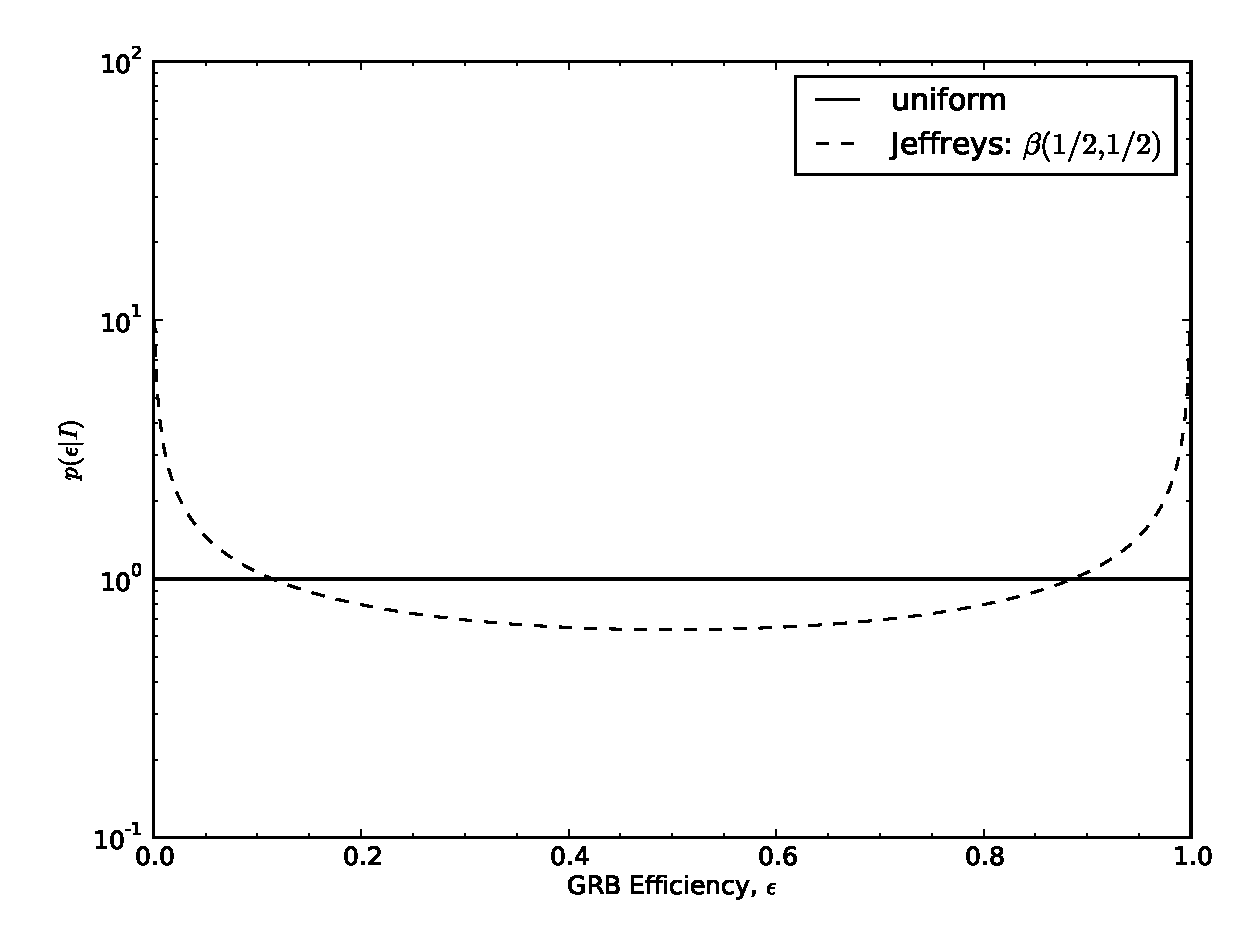
\includegraphics[width=\linewidth]{efficiency_prior.eps}}\label{fig:priors}
%   \caption{Priors}
%   \end{figure}

% \subsection{A Note On Implementation} %
%{\tt EMCEE}~\cite{2013PASP..125..306F}.
% Points are sampled from the joint distribution $p(\theta,\epsilon)$,
% where equation~\ref{eq:rate2angle} is used to derive the corresponding
% value of $\cbcrate$ for a given $(\theta,\epsilon)$.  We then obtain
% the marginal distribution $p(\theta)$ via \ac{KDE} of the
% $\theta$-samples.  The mode of the \ac{KDE} yields the maximimum a
% posteriori estimate for the measurement, and the upper and lower
% bounds are found from the 95\% confidence interval around the median
% of the samples.


\section{Prospects For Beaming Angle Constraints With Advanced LIGO}
We now demonstrate the derivation of the rate posterior $p(\cbcrate)$
and the subsequent transformation to the beaming angle posterior
$p(\theta)$.  We consider four \ac{GW} observation scenarios with
\ac{aLIGO} based on the work in~\cite{Aasi:2013wya}.  An observing
scenario essentially consists of an epoch of \ac{aLIGO} operation,
which defines an expected search sensitivity (i.e., \BNS{} horizon
distance $\dhor$) and observation time $T$; as well as an assumption
on the rate of \BNS{} coalescence in the local universe $\cbcrate$.
Each observing scenario ultimately results in an expectation for the
number of observed \acp{GW} from \BNS coalescences.  For this study,
we consider two operation epochs: the 2016 and 2022+ scenarios
described in~\cite{Aasi:2013wya} and we assume the `realistic rate'
for $\cbcrate$ as described in~\cite{rates_paper}.

Our first goal is to establish the expected number of detections in
each scenario.  Given the observation time and horizon distance of the
observation epoch we first compute the 4-volume accessible to the
analysis,
%
\begin{equation}
    \label{eq:search_volume}
    V_{\mathrm{search}} = \frac{4}{3}\pi \left(\frac{\dhor}{2.26}\right)^3 \times \gamma T,
\end{equation}
%
where the factor 2.26 arises from averaging over source sky location
and orientation, $T$ is the observation time and $\gamma$ is the
\emph{duty cycle} for the science run.  Following~\cite{Aasi:2013wya},
we take $\gamma=0.5$.  For comparison, during the first observing run
of \ac{aLIGO}, the two interferometers observed in coincidence
achieving $\gamma_{\mathrm{coinc}} = 0.41$.  Where there is a range in
the horizon distances quoted in~\cite{Aasi:2013wya} to account for
uncertainty in the sensitivity of the early configuration of the
detectors, we use the arithmetic mean of the lower and upper bounds
when computing the search volume.  Table~\ref{table:scenarios} lists
the details of each observing scenario.
%
\dwnote{We probably want to consider exactly which observing scenarios
  we include here; it's reasonably trivial to generate new ones from
  the code.}%
%
\begin{table}
\centering
\begin{tabular}{lcccc}
  \toprule
  Epoch & $T$ & \dhor & $V_{\mathrm{search}}$ & $N$ \\
        & [yr] & [Mpc] & [$\ee{6} \mpc³\,\yr^{-1}$ & \\
  \colrule
  2015 - 2016 & 0.25 & 73 & 0.45 & 0 \\
  2016 - 2017 & 0.5 & 100 & 1.3 & 1\\
  2017 - 2018 & 0.75 & 145 & 6.5 & 3\\
  2019 + & 1 & 200 & 20 & 10\\
  2022 + & 1 & 200 & 40 & 20\\
  \botrule
\end{tabular}
\caption{Advanced detector era observing scenarios considered in this work.
    $T$ is the expected duration of the science run and $\dhor$ is the \BNS horizon distance for the sensitivity expected to be achieved at the given epoch.
$V_{\mathrm{search}}$ is the sensitive volume of the search, defined by equation~\ref{eq:search_volume}, and $n$ is the expected number of \ac{GW} detections.
    Note that the quoted search volume accounts for a network duty cycle of $\sim 50\%$.
    These scenarios are derived from those detailed in~\cite{Aasi:2013wya}.
    \label{table:scenarios}}
\end{table}
%

\subsection{Posterior Results}
Figure~\ref{fig:aligorate} shows the rate posteriors resulting from
the observations described in table~\ref{table:scenarios} for the
expected early \ac{aLIGO} sensitivity in the 2016 epoch (broad, solid
curve) and the nominal design sensivity (narrow, dashed curve), using
the `realistic' rate $\cbcrate=10^{-6}$\,Mpc$^{-3}$yr$^{-1}$.
%\footnote{The curves corresponding to the
%`high' rate show similar qualitative behaviour and are not included here in the
%interests of brevity.}  
We now use curves such as these together with the prior distributions
described in section~\ref{sec:rate_posterior} and the observed rate of
\acp{sGRB} (as described in section~\ref{sec:sgrbs}, we use
$\grbrate=10$\,Gpc$^{-3}$yr$^{-1}$~\cite{Nakar:2007yr,Dietz:2010eh})
to derive the corresponding beaming angle posteriors.

\begin{figure}
\centering
{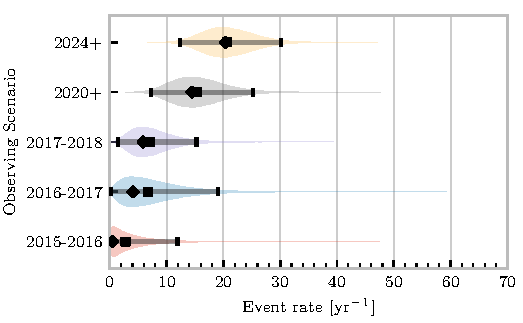
\includegraphics[width=\linewidth]{rate_posteriors_violin.pdf}}
\caption{Posterior probability distribution for the rate of \BNS
  coalescence assuming the scenarios A (red shading) \& B (blue shading)
  detection scenarios. The 95\% confidence interval is represented with a horizontal line through the centre of the plot, with vertical lines delineating the 2.5\% and 97.5\% percentiles; the median is represented by a square marker, and the maximum \latin{a posteriori} (\ac{MAP}) value is denoted by a diamond.  \dwnote{* TODO I should update these plots so that they reflect the correct scenario names.}
  \label{fig:aligorate}}
\end{figure}

\subsubsection{Validation}
Before we derive beaming angle posteriors corresponding to the
aforementioned observing scenarios, it is useful to establish some
form of validation for our procedure.  This validation is performed by
first selecting values of the beaming angle, the \ac{sGRB} efficiency,
and the rate of \BNS coalescence.  We choose $\theta=30^{\circ}$,
$\epsilon=0.5$, and the `realistic' rate
$\cbcrate = 10^{-6}$\,Mpc$^{-3}$yr$^{-1}$.  We then compute the value
of the \ac{sGRB} rate that would correspond to these parameter
choices.  Finally, we simply use this \emph{artificial} value for
$\grbrate$ in equation~\ref{eq:beam_posterior} when we compute the
posterior on the beaming angle, with the understanding that the
resulting posterior should yield an inference consistent with the
`true' value $\theta=30^{\circ}$.
%
\begin{figure}%[H]
\centering
{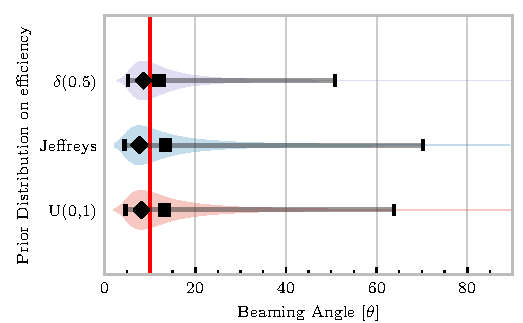
\includegraphics[width=\linewidth]{O1_injections_violin.pdf}}
\caption{Beaming angle posteriors with different priors.
    An artificial \ac{sGRB} rate has been imposed in order that the target value of the beaming angle is $\theta = 30^{\circ}$.
    These posteriors are based on the O1 observing scenario (see table~\ref{table:scenarios}).
    \dwnote{* TODO I should update these plots so that they reflect the correct scenario names.}
    \label{fig:injjetposterio2016}}
\end{figure}
%
\begin{figure}%[H]
\centering
{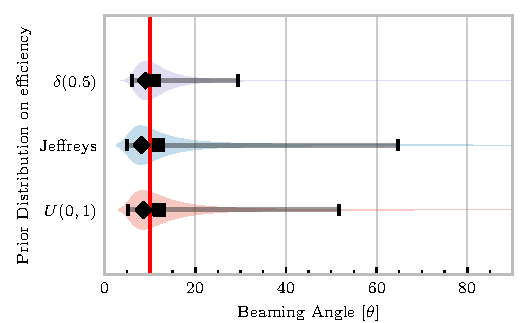
\includegraphics[width=\linewidth]{O2_injections_violin.pdf}}
\caption{Beaming angle posteriors with different priors.
    An artificial \ac{sGRB} rate has been imposed in order that the target value of the beaming angle is $\theta = 30^{\circ}$.
    These posteriors are based on the O2 observing scenario (see table~\ref{table:scenarios}).
    \dwnote{* TODO I should update these plots so that they reflect the correct scenario names.}
    \label{fig:injjetposterio2022}}
\end{figure}
%
Figures~\ref{fig:injjetposterio2016} and~\ref{fig:injjetposterio2022}
show the beaming angle posteriors which result from this analysis for
the 2016 and 2022 scenarios respectively.  Unsurprisingly, the most
accurate constraints arise when we already have the tightest possible
constraints on the \ac{sGRB} efficiency, $\epsilon$.  That is, the
beaming angle posterior arising from the $\delta$-function prior on
$\epsilon$ is the narrowest, yielding the shortest possible confidence
interval.  It is well worth remembering, however, that had we been
incorrect regarding the value of $\epsilon$ when using the
$\delta$-function prior, the result would be significantly biased and
our inference on the beaming angle would be incorrect.  This
highlights the necessity of building a suitable representation of our
ignorance into the analysis.  Finally, we note that the results from
the uniform and $\beta$-distribution priors are broadly equivalent.


\subsubsection{Jet Angle Posteriors From Observing Scenarios}
Figures~\ref{fig:jetposterior2016} and~\ref{fig:jetposterior2022} show
the beaming angle posteriors obtained for our two detection scenarios.
\footnote{A note on implementation: rather than directly evaluating
  the beaming angle posterior in equation~\ref{eq:beam_posterior} we
  choose to sample points from the posterior using a Markov-Chain
  Monte-Carlo algorithm, implemented using the python package
  \texttt{PyMC3}~\cite{salvatier2016probabilistic}.}
Since it is a common assumption in related literature, we also now
include a prior on the \ac{sGRB} efficiency which dictates that all
\BNS produce a \ac{sGRB}, $p(\epsilon|I)=\delta(\epsilon=1)$, as well
as our previous strong $\delta$-function prior.  For the 2016 scenario
where inferences are somewhat weak (i.e., broad posteriors) due to the
sparcity of \ac{GW} detections, the uncertainties are large enough
that the results from each prior are broadly consistent.  In the 2022
scenario, where the posterior is more peaked, it is clear that the
strong $\delta$-function priors lead to inconsistent inferences on the
\ac{sGRB} beaming angle.  The much weaker uniform and $\beta$
distributions, by contrast, are again largely consistent with each
other yielding more conservative and robust results, as well as being
a more representative expression of our state of knowledge.  The
inferences drawn from each scenario and each prior are summarised in
terms of the maximum \emph{a posteriori} measurement and the 90\%
confidence interval around the maximum in
table~\ref{table:aligo_beam_inference}.

\begin{figure}
\centering
{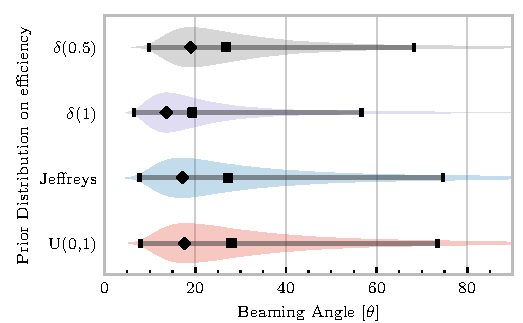
\includegraphics[width=\linewidth]{O1_beaming_posteriors_violin.pdf}}
\caption{Beaming angle posteriors using different priors on \ac{sGRB} efficiency $\epsilon$ in observing scenario A.
  \dwnote{* TODO I should update these plots so that they reflect the correct scenario names.}
    \label{fig:jetposterior2016}}
\end{figure}

\begin{figure}
\centering
{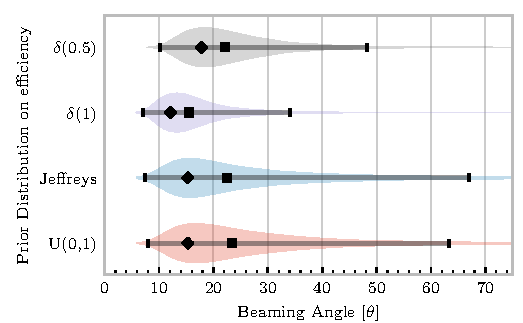
\includegraphics[width=\linewidth]{O2_beaming_posteriors_violin.pdf}}
  \dwnote{* TODO I should update these plots so that they reflect the correct scenario names.}
\caption{Beaming angle posteriors using different priors on \ac{sGRB} efficiency $\epsilon$ in observing scenario B.
    \label{fig:jetposterior2022}}
\end{figure}

\begin{table}
\centering
\begin{tabular}{l c c c c }
\toprule
% &\multicolumn{4}{c}{Prior} \\
Scenario & $\delta(\epsilon=0.5)$ & $\delta(\epsilon=1)$ & $U(0,1)$ & $\beta(\frac{1}{2},\frac{1}{2})$\\
\cline{1-1}\cline{2-5}
\colrule
2016  & $4.10^{+6.67}_{-1.16}$ & $2.90^{+4.34}_{-0.82}$ &\ $6.50^{+68.37}_{-3.00}$ & $6.20^{76.34}_{-2.26}$ \\
2022 & $6.20^{+0.99}_{-0.73}$ & $4.30^{+0.79}_{-0.46}$ & $7.00^{+65.99}_{-2.11}$ & $6.90^{+72.85}_{-2.29}$ \\
\botrule
\end{tabular}
\caption{Summary of the beaming angle inferences for each prior in the two observing scenarios considered in this work.
    Point estimates are the maximimum a posteriori estimates and errors correspond to the $90\%$ confidence interval around the maximum.
    \label{table:aligo_beam_inference}}
\end{table}

%   \begin{figure}
%   \centering
%   {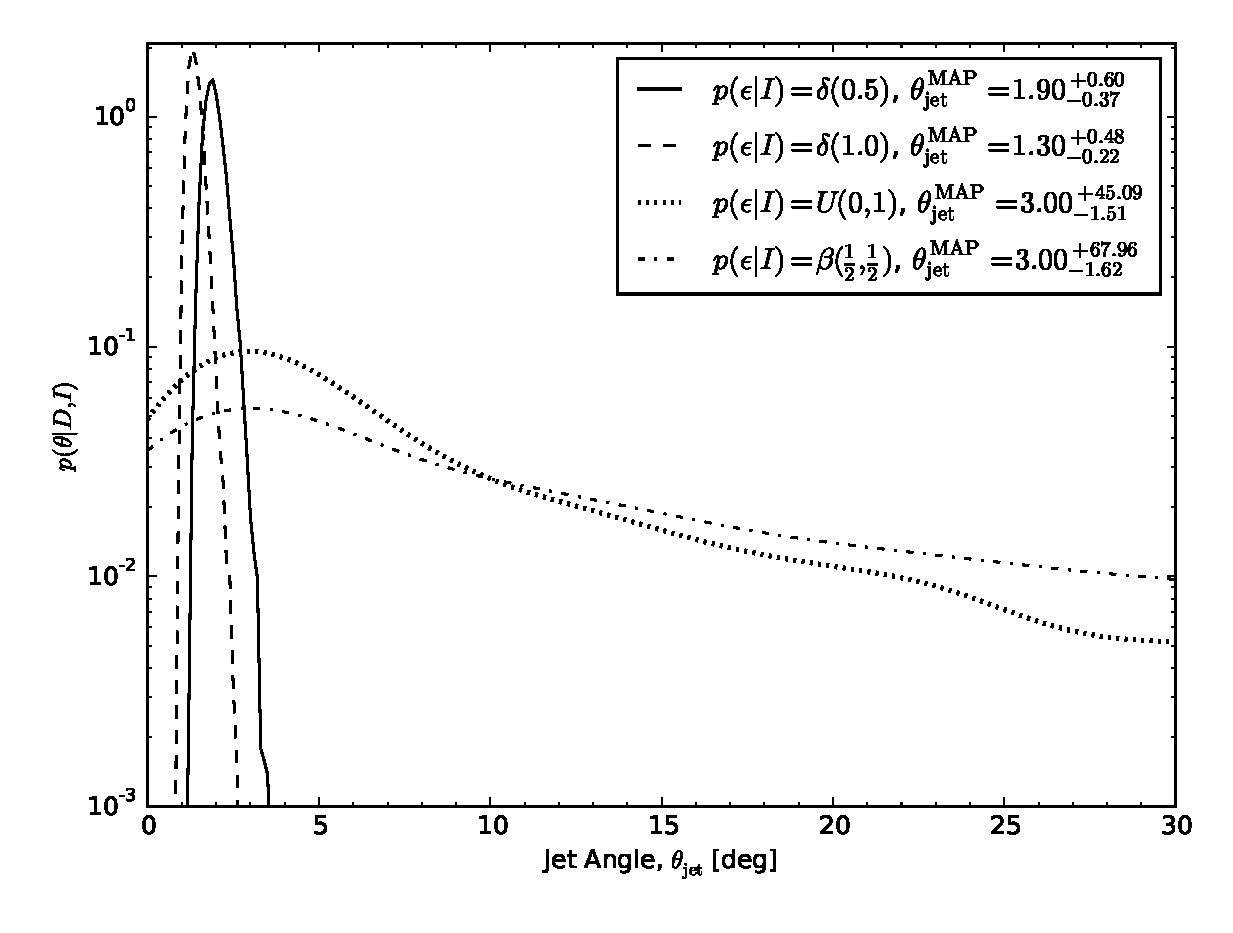
\includegraphics[width=\linewidth]{jet_angle_posterior_aligo_2016_high_real.eps}}
%   \caption{ADE 2016 jet angle posterior, high rate}
%   \end{figure}
%
%   \begin{figure}
%   \centering
%   {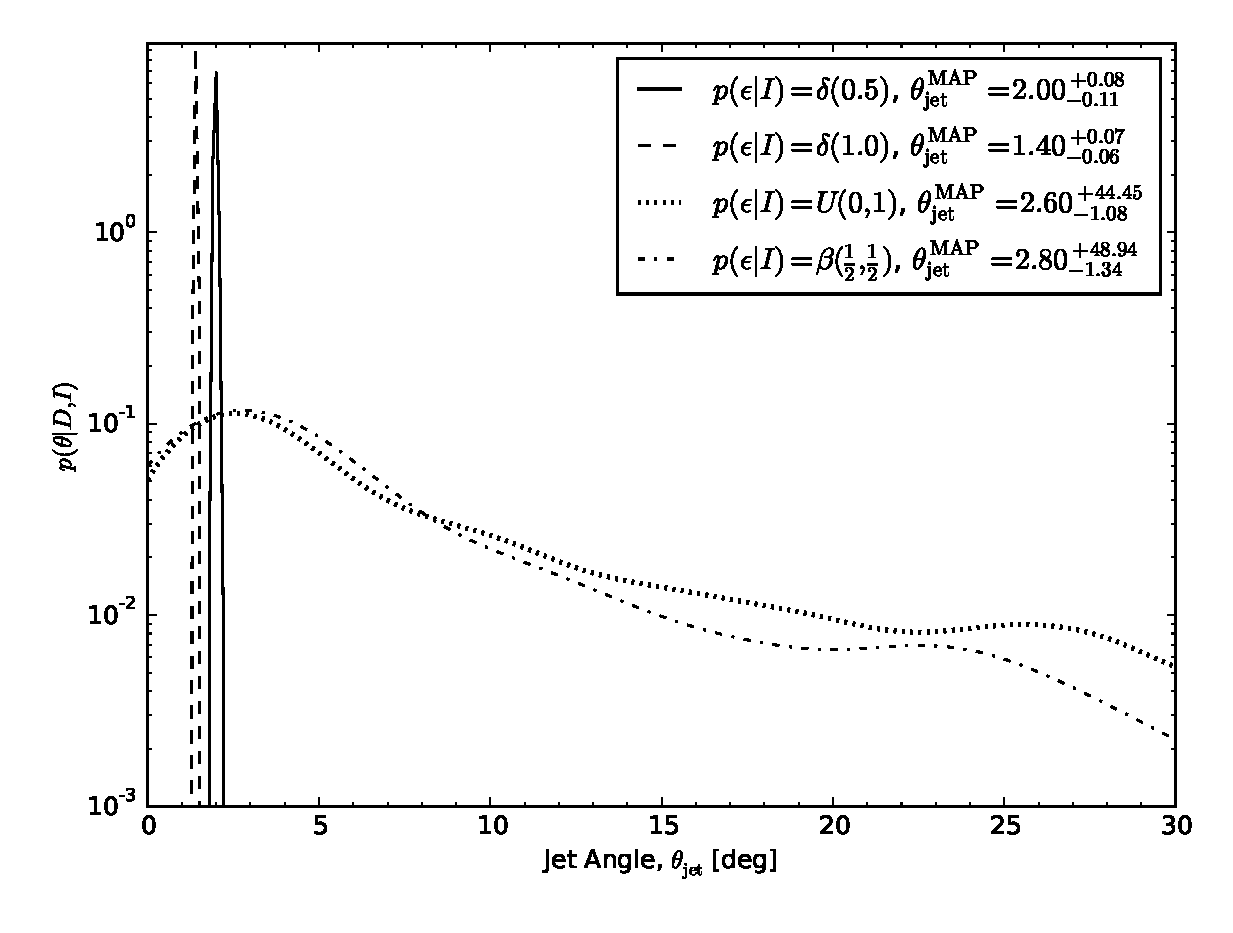
\includegraphics[width=\linewidth]{jet_angle_posterior_aligo_2022_high_real.eps}}
%   \caption{ADE 2022 jet angle posterior, high rate}
%   \end{figure}

\section{Beaming Angle Constraints With No \ac{GW} Detections}
\label{sec:beaming_limits}
Our proposed approach is also valid in the regime where no \ac{GW} signals from \BNS coalescence have been observed.
In this case, the procedure is identical: construct the posterior probability density function on the \BNS coalescence rate, transform to the joint posterior on the beaming angle and \ac{sGRB} efficiency, $\epsilon$, and marginalise over the nuisance parameter $\epsilon$ to yield the posterior on the beaming angle.
Now, however, rather than quoting the maximum a posteriori estimate, together with some confidence interval, we simply integrate the beaming angle posterior from $\theta=0$ until we reach that value which contains some desired confidence.
Thus, we obtain an upper limit on the beaming angle, analogous to the rate upper limits set by past LIGO observations~\cite{Colaboration:2011np}.

In this section, we demonstrate the procedure using the \BNS coalescence rate measurements from the final science run of LIGO, prior to the upgrade to \ac{aLIGO}.

\arw{Here, and elsewhere, we should change to using O1 upper limits from the O1 BNS/NSBH paper~\cite{Abbott:2016ymx}. These are $\cbcrate=1.21\times 10^{-5}$\,Mpc$^{-3}$yr$^{-1}$ for `low spin' and $\cbcrate=1.26\times 10^{-5}$\,Mpc$^{-3}$yr$^{-1}$ for `high spin'.}


%   \subsection{Constructing The Rate Posterior} Our first objective is the
%   construction of the rate posterior.  Since our ultimate goal here is to derive a
%   beaming angle posterior based on initial LIGO observations, it is convenient to
%   adopt the same approach to constructing the rate posterior that was used in past
%   analyses.  Following~\cite{Biswas09,BradyFairhurst08}, the posterior on the
%   binary coalescence rate may be determined from the loudest event in the \ac{GW}
%   analysis and takes the form,
%   %Specifically, for a foreground event rate due to  binary coalescence
%   %$\cbcrate$, the probability of obtaning no events with ranking statistic $\rho$
%   %greater than the observed loudested event $\rhostar$ is,
%   %
%   %\begin{equation} P_F(\rhostar | \cbcrate, C_L, T) = e^{-\cbcrate C_L(\rhostar)
%   %T}, \end{equation}
%   %
%   %where $C_L(\rhostar)$ is the total luminosity to which the search is sensitive
%   %and $T$ is the duration of the search.  The overall probability of obtaining no
%   %events with ranking statistic $\rho>\rhostar$ is the product of obtaining no
%   %such events from foreground \emph{and} the probability of obtaining no such
%   %events from the background in the detector, denoted $P_B(\rhostar)$,
%   %
%   %\begin{equation} P(\rhostar|\cbcrate,I) = P_B(\rhostar|I)e^{-\cbcrate
%   %C_L(\rhostar) T} \end{equation}
%   %
%   %Using a uniform prior on $\cbcrate$ and inverting the overall probability with
%   %Bayes' theorem, we arrive at,
%   %
%   \begin{equation}\label{eq:loudestEventPosterior} p(\cbcrate | C_L({\rhostar}),
%   T, \Lambda) \propto p(\cbcrate) \left[ \frac{1+\Lambda C_L(\rhostar)
%   T}{1+\Lambda}\right] e^{-\cbcrate C_L(\rhostar) T}, \end{equation}
%   %
%   where $p(\cbcrate)$ is the prior probability distribution on the rate, assumed
%   to be uniform, $C_L(\rhostar)$ is the total luminosity to which the search is
%   sensitive, and $T$ is the observation time.  The quantity $\Lambda$ is
%   essentially the relative likelihood that the loudest event arose from a \ac{GW}
%   signal to the likelihood of background.  See section\,3
%   of~\cite{BradyFairhurst08} for the derivation of this distribution and the
%   quantities involved.
%
%   We can now use the published upper limits on the rate of \BNS coalescence to
%   re-derive the full rate posterior.  The upper limit on the binary coalescence
%   rate at confidence $\alpha$ is found by integrating the rate posterior from zero
%   to $\alpha$.  Assuming a uniform prior on the rate $\cbcrate$ and using the rate
%   posterior given by equation~\ref{eq:loudestEventPosterior}, the upper limit on
%   the rate $\cbcrate_{\alpha}$ is given by equation 21 in~\cite{BradyFairhurst08}:
%   %
%   \begin{equation}
%   1-\alpha =  e^{-\cbcrate_{\alpha} C_L(\rhostar)T)}
%   \left[ 
%   1+ \left(\frac{\Lambda}{1+\Lambda}\right) \cbcrate_{\alpha} T C_L(\rhostar)
%   \right ].
%   \label{eq:rateIntegral}
%   \end{equation}
%   %
%   In the event that no \ac{GW} signal has been observed and the loudest event is
%   umabiguously due to background noise fluctuations, we are in the limit in which
%   $\Lambda \rightarrow 0$.
%   In this case, we simply have,
%   \begin{equation}
%   C_L(\rhostar)T = -\frac{\log(1-\alpha)}{\cbcrate_{\alpha}},
%   \end{equation}
%   %
%   %and the value of $\cbcrate$ can be taken straight from the literature
%   %\footnote{Note
%   %that this procedure necessarily confines our jet angle inferences based on
%   %progenitor systems for which the rate upper limits are available.  Given that
%   %the binary coalesence rate limits are quoted for canonical binary neutron star
%   %and neutron star-black hole systems, both plausible sGRB progenitors, this
%   %simply means our inferences on the jet angle are specific to each system and
%   %treated separately.}
%   %
%
%   \begin{figure}
%   \centering
%   %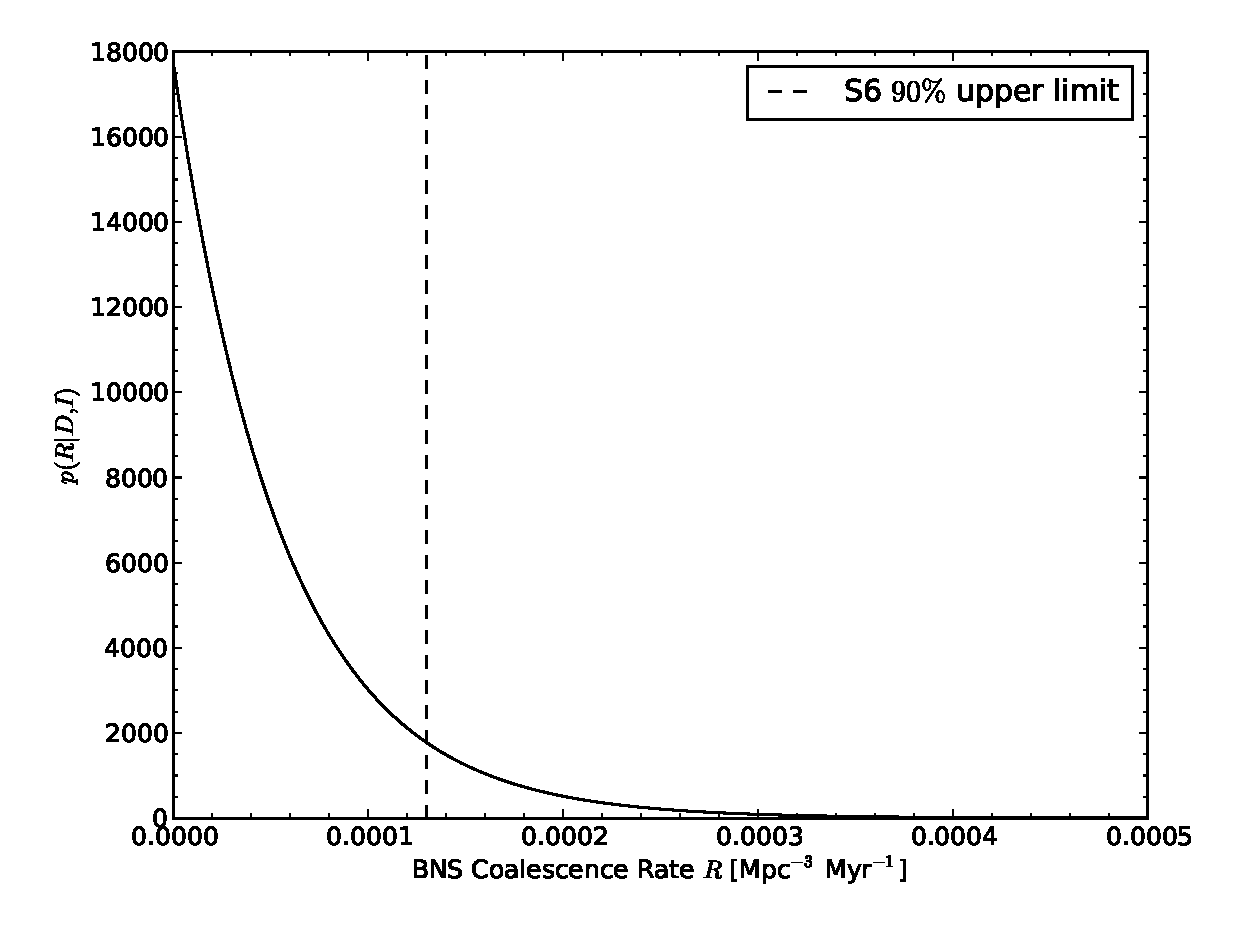
\includegraphics[width=\linewidth]{S6_rate.eps}
%   \caption{Posterior on the rate of \BNS coalescence based on obsevations taken during the S6/VSR2,3 science runs of initial LIGO and Virgo~\cite{Colaboration:2011np}.
%       The posterior is constructed using the loudest event procedure~\cite{Biswas09,BradyFairhurst08} and reconstructed from published upper limits (see text).
%       \label{fig:s6rate}}
%   \end{figure}
%
%   Using the most stringent 90\% confidence upper limit from \ac{GW} observations on the rate of binary neutron star coalescences to date, $\cbcrate^{90\%}_{{\rm BNS}} = 1.3\times 10^{-4}$\,Mpc$^{-3}$yr$^{-1}$~\cite{Colaboration:2011np}, gives $C_L(\rhostar)T=17712$.
%   The full rate posterior from~\cite{Colaboration:2011np} is then found by inserting this value and $\lambda=0$ in equation~\ref{eq:loudestEventPosterior}.
%   The result is shown in figure~\ref{fig:s6rate}.
%
%
%   %Similarly, for NS-BH systems,  $\cbcrate^{90\%}_{{\rm
%   %nsbh}} = 3.1\times 10^{-5}$\,Mpc$^{-3}$yr$^{-1}$ gives $C_L(\rhostar)T=74277$.
%   %The posteriors on the rates, assuming these values and $\Lambda=0$, are shown in
%   %figure~\ref{fig:reconstructedRatePosterior}.  

%\subsection{Results}

Figure~\ref{fig:s6angle} shows the four posteriors on the beaming angle, corresponding to the four priors on the \ac{sGRB} efficiency, $\epsilon$, using the rate posterior obtained from \ac{GW} measurements in the final science run of the first generation of ground based \ac{GW} detectors.
In this non-detection scenario, we choose to compute the 95\% confidence \emph{upper} limit on the beaming angle,
\begin{equation}
    \label{eq:beaming_upper_limit}
    0.95 = \int_0^{\theta^{\mathrm{ul}}} p(\theta|D,I)~\diff \theta
\end{equation}
%
We see that here, where the rate posterior is rather uninformative, the results are dominated by the uncertainty in $\epsilon$: there are substantive differences in the beaming angle upper limits yielded by the uniform ($U(0,1)$) and $\beta$-distribution priors, while the $\delta$-function priors yield dramatically different upper limits.
Indeed, the most stringent (and mutually incompatible) upper limits are obtained using the strong $\delta$-function priors.
In fact, these beaming angle upper limits are also incompatible with the values of $3^{\circ}\mbox{-}8^{\circ}$ that have been inferred from observations of jet breaks in \ac{sGRB} afterglows~\cite{Fong:2013lba,2006MNRAS.367L..42P, 2012A&A...538L...7N}.
Recall, however, from the discussion in section~\ref{sec:sgrbs} that we interpret the beaming angle inference from our rate measurements as the upper bound on the mean of a population of beaming angles.
It would, therefore, seem premature to conclude that there is tension in these results; instead, we can only state that either the population of \acp{sGRB} have a distributio of beaming angles with some finite width or that the fraction of \BNS mergers which yield a \ac{sGRB} is smaller than 0.5.

It is also interesting to compare these upper limits on the beaming angle with those in~\cite{2013PhRvL.111r1101C}, where the upper limit on the rate itself is used as a constraint (rather than transforming the posterior).
This has the important implication that the constraint thus obtained is the \emph{smallest} angle consistent with the rate:
%
\begin{equation}
    1 - \cos \theta \geq \frac{\grbrate}{\epsilon \cbcrate^{\mathrm{ul}}},
\end{equation}
%
where $\cbcrate^{\mathrm{ul}}$ is the \emph{upper limit} on the \BNS rate.
The same idea is used in~\cite{Clark:2014jpa} to estimate beaming constraints in the advanced detector era.
Thus, when comparing the constraints in e.g.,~\cite{2013PhRvL.111r1101C} and the upper limits obtained from the transformed posterior (i.e., equation~\ref{eq:beam_posterior} and figure~\ref{fig:s6angle}), one should remember that they are quite different quantities.
There are two other noteworthy differences between~\cite{2013PhRvL.111r1101C} and this work: (i) the rate upper limit is computed based on the sensitivity of the initial LIGO-Virgo network (see e.g.,~\cite{BradyFairhurst08}), which gives $\cbcrate=4.5\times 10^{-4}$\,Mpc$^{-3}$yr$^{-1}$ (as compared with $\cbcrate=1.3 \times 10^{-4}$\,Mpc$^{-3}$yr$^{-1}$ from the analysis in~\cite{Colaboration:2011np}); and (ii) it is implicitly assumed that \emph{all} \BNS mergers yield an \ac{sGRB}.
That is, there is no factor or $\epsilon$ to account for the unknown fraction of mergers which successfully launch an \ac{sGRB} jet.
With these differences noted, the lower bound on the beaming angle is found to be $\theta \geq 0.8^{\circ}$, as compared with our 95\% confidence upper limit $\theta^{\mathrm{ul}}=1.94^{\circ}$ when assuming $\epsilon=1$.

\begin{figure}
\centering
%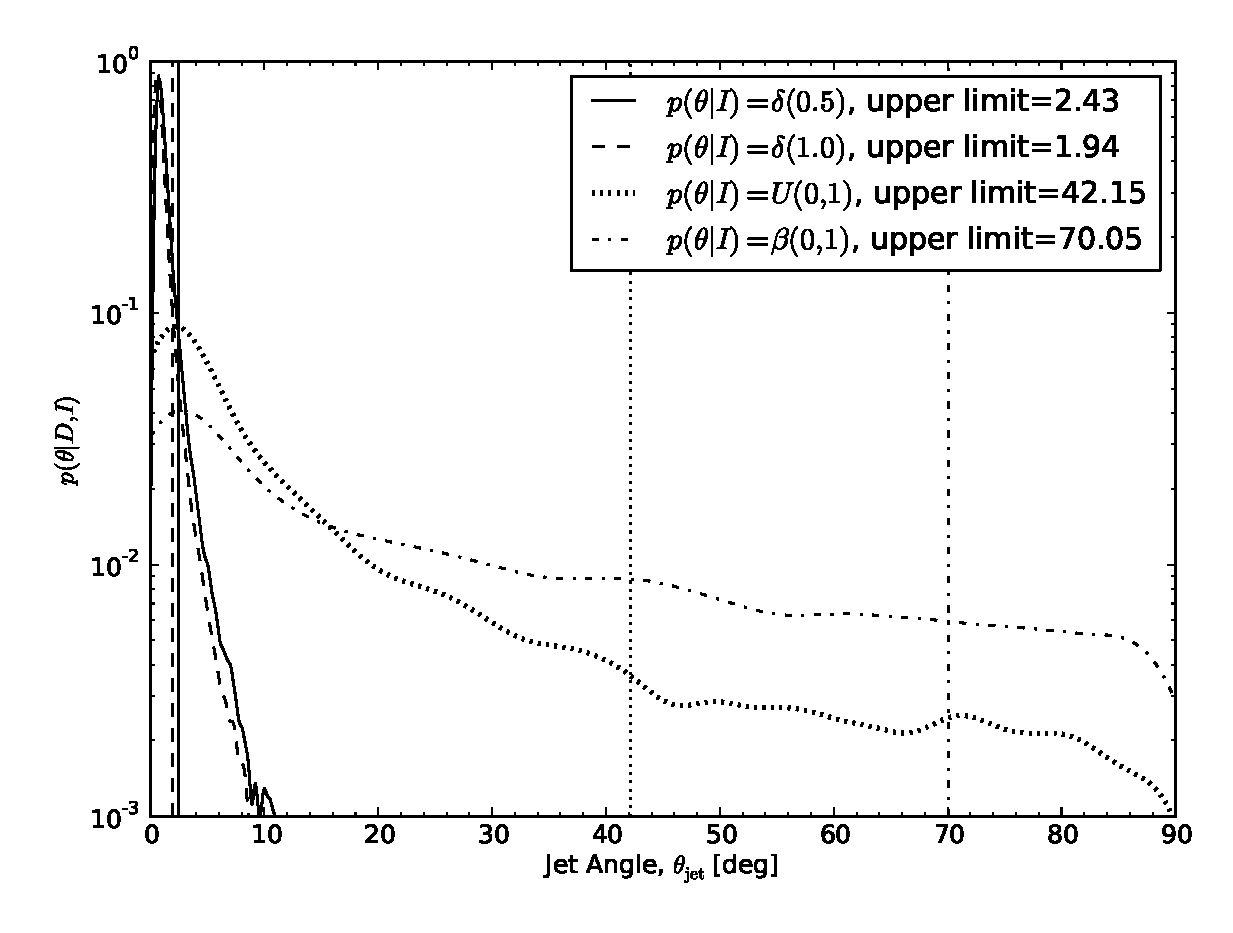
\includegraphics[width=\linewidth]{jet_angle_posterior_iligo.eps}
\caption{Beaming angle posterior using the rate posterior (see figure~\ref{fig:s6rate}) obtained from S6/VSR2,3 observations~\cite{Colaboration:2011np}.
    Priors on $\epsilon$ now dominate our results.
    \label{fig:s6angle}}
\end{figure}

\begin{figure}
\centering
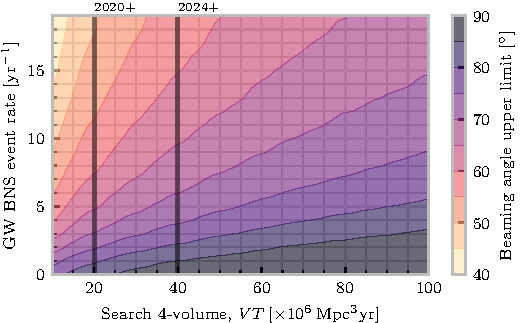
\includegraphics[width=\linewidth]{volume_v_nevents.pdf}
%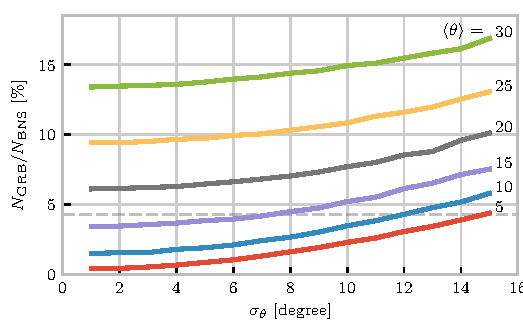
\includegraphics[width=\linewidth]{color_relativenumber.pdf}
\caption{\label{fig:volumevevents} The median beaming angle for different observed volumes and numbers of observed events.}

    % \centering
    % 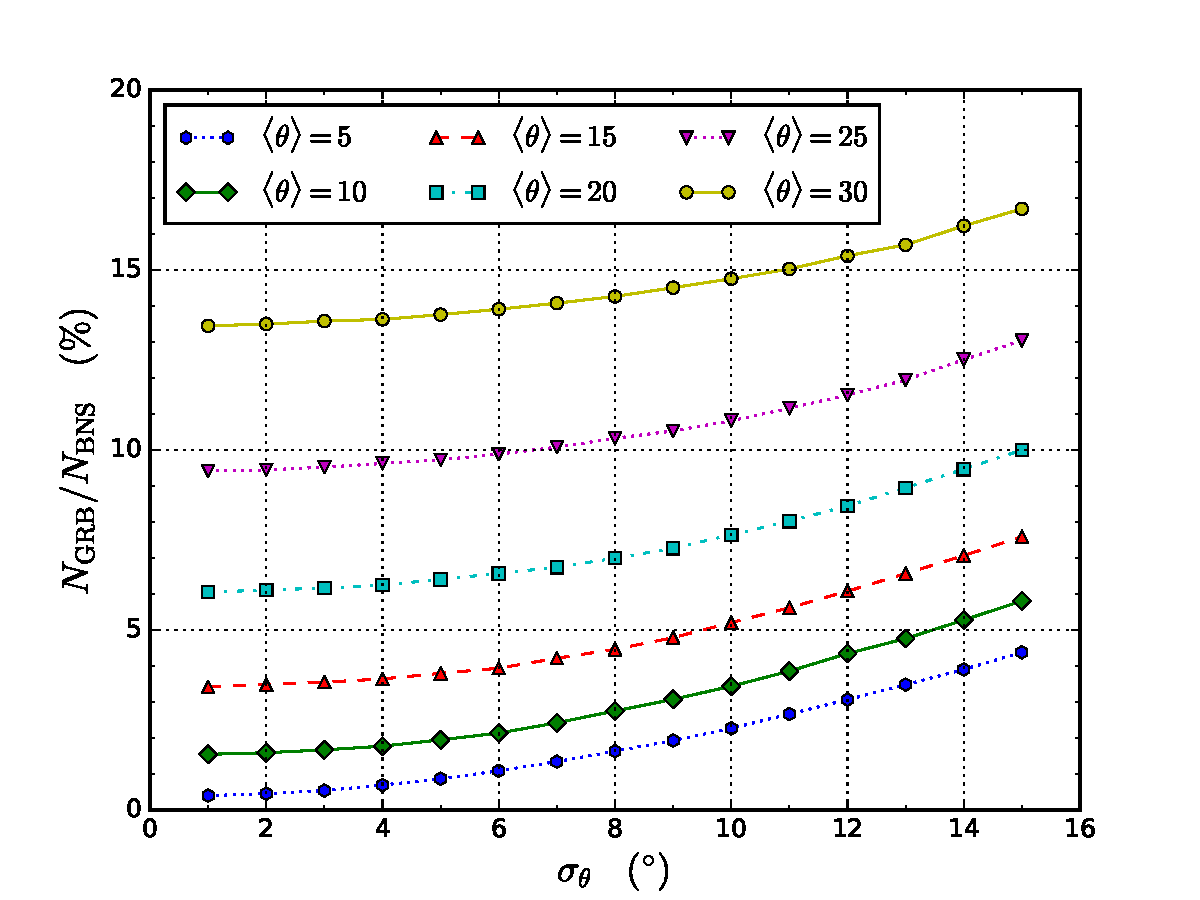
\includegraphics[width=\linewidth]{figure1.pdf}
    % \caption{Expected ratio of observed SGRBs and binary coalescences for different distributions on the SGRB beaming angle.
    %     For a series of jet angle population means, $\langle \theta \rangle$, we plot this ratio as a function of the distribution width, $\sigma_{\theta}$.
    %     All jet angle distributions are normal, truncated at $(0, 90]$ degrees.
    %     \label{fig:thetapop}}
\end{figure}

%%% EDITED TO HERE %%%
\section{Conclusion}

\begin{comment}

\appendix


\section{Jacobian Calculation}
This doesn't need to be in the publication, these are just notes for James'
benefit and possibly verification.

\begin{equation}
\cbcrate=\frac{\grbrate}{\epsilon(1-\cos \theta)},
\end{equation}

\begin{equation}
p(\theta) = \int_{\epsilon} p(\theta,\epsilon)~\diff \epsilon,
\end{equation}

\begin{equation}
p(\theta,\epsilon) = p(\cbcrate,\epsilon)
\left\lvert\left\lvert
\frac{\partial(\cbcrate,\epsilon)}{\partial(\theta,\epsilon)}
\right\rvert\right\rvert,
\end{equation}

% Increase matrix line spacing
\begingroup
\renewcommand*{\arraystretch}{1.5}

% matrix:
\begin{equation}
\frac{\partial (\cbcrate,\epsilon)}{\partial(\theta,\epsilon)} =
\begin{bmatrix}
\frac{\partial \cbcrate}{\partial \theta} & \frac{\partial \cbcrate}{\partial \epsilon} \\
\frac{\partial \epsilon}{\partial \theta} & \frac{\partial \epsilon}{\partial \epsilon}
\end{bmatrix}.
\end{equation}

% end line spacing increase
\endgroup

\begin{eqnarray}
\frac{\partial \cbcrate}{\partial \theta} & = &
-\frac{\grbrate\sin\theta}{\epsilon(\cos\theta - 1)^2}\\
\frac{\partial \cbcrate}{\partial \epsilon} & = &
\frac{\grbrate}{\epsilon^2(\cos\theta-1)}\\
\frac{\partial \epsilon}{\partial \theta} & = &
-\frac{\grbrate\sin\theta}{\cbcrate(\cos\theta-1)^2}\\
\frac{\partial \epsilon}{\partial \epsilon} & = & 1\\
\end{eqnarray}

\begin{eqnarray}
\left\lvert
\frac{\partial(\cbcrate,\epsilon)}{\partial(\theta,\epsilon)}
\right\rvert & = & \frac{\partial \cbcrate}{\partial \theta}
\frac{\partial \epsilon}{\partial \epsilon} - \frac{\partial \cbcrate}{\partial
\epsilon}\frac{\partial \epsilon}{\partial \theta} \\
& = & -\frac{2\sin\theta}{\epsilon(\cos\theta-1)^2}
\end{eqnarray}
%
Finally:
\begin{equation}
\left\lvert\left\lvert
\frac{\partial(\cbcrate,\epsilon)}{\partial(\theta,\epsilon)}
\right\rvert\right\rvert = \frac{2\grbrate\sin\theta}{\epsilon(\cos\theta-1)^2} 
\end{equation}



\section{Null-detection Jet Angle Posteriors With Different Priors}

\end{comment}

\bibliography{grb_beams_paper}

\end{document}
